%%%%%%%%%%%%%%%%%%%%%%%%%%%%%%%%%%%%%%%%%%%%%%%%%%%%%%%%%%%%%%%%%%%%%%%%%%%%%%%
%%%%%%%%%%%%%%%%%%%%%%%%%%%%%%%%%%%%%%%%%%%%%%%%%%%%%%%%%%%%%%%%%%%%%%%%%%%%%%%
%%%%  CHAPTER 5 
%%%%%%%%%%%%%%%%%%%%%%%%%%%%%%%%%%%%%%%%%%%%%%%%%%%%%%%%%%%%%%%%%%%%%%%%%%%%%%%
%%%%%%%%%%%%%%%%%%%%%%%%%%%%%%%%%%%%%%%%%%%%%%%%%%%%%%%%%%%%%%%%%%%%%%%%%%%%%%%
\chapter{Compensated optical lattice potential}
\label{chap:compensated-optical-lattice}


One of the most important aspects of the work presented in this thesis has been
the design and construction of the potential in which our experiments take
place.   In previous chapters we have referred to ultracold atoms in optical
lattices as a nearly ideal realization of the Hubbard model.   In fact, there
are important differences between ultracold atoms in optical lattices and
idealized models.    

To start with, optical lattices are created with finite laser beams, and thus
the value of the lattice depth is never constant throughout the sample.      In
addition, when using ultracold atoms one is forced to use an overall confining
potential, to achieve large enough densities close to one particle per site
(half-filling) such that the effects of correlations between particles become
manifest.  An illustration of these ideas is shown in
Fig.~\ref{fig:comp-uncomp}. 
\begin{figure}
    \centering
\includegraphics[width=\textwidth]{../illustrations/lattice/comp+uncomp-inhom.png}
\caption{\small In an ideal system (left) a lattice is homogeneous and flat,
extending to infinity.  For a finite number of particles the density would go
to zero, as the gas continues to expand in the lattice.   For real Gaussian
beams (center), the lattice is inhomogeneous.  Notice that the inhomogeneity of
the lattice beams results in a small amount of confinement (curvature of lower
envelope of the potential), but not sufficient to increase the density
significantly.   Additional confinement (right) must be provided to achieve the
necessary densities with a finite number of particles.  } 
\label{fig:comp-uncomp}
\end{figure}
In recent years there has been significant work in trying to make
``square-well'' potentials, that are flat but have very steep
walls~\cite{liang20091,PhysRevLett.110.200406}.  In such potentials one could
reach densities near half-filling and have a homogeneous lattice depth at the
same time.  This approach, to our knowledge, has not yet been realized with
optical lattices.

Experiments in lattices have traditionally dealt with at least one of the
problems stated above: the inhomogeneity of the lattice depth.    Typically,
experiments use lattice beam waists that are large comparable to the size of
the system.   An additional Gaussian beam (or arrangement of beams) with
smaller waists provides the external confinement and determines the size of the
system.   This approach has the advantage that the lattice depth, being nearly
constant throughout the extent of the sample, results in Hubbard parameters $t$
and $U$ that are also nearly constant throughout the sample. In any case, the
density distribution of the atoms still remains inhomogeneous due to the
external confinement, and that presents a problem for the interpretation of
bulk measurements.   Furthermore, the traditional setup (large beam waist +
additional confinement)  has a disadvantage that has to do with the possibility
of continuing to evaporatively cool the atoms once they are loaded into the
lattice potential.  

The field of ultracold atomic physics has built its success by exploiting the
power of two very effective atom cooling techniques, laser cooling and
evaporative cooling.  The former makes use of dissipative forces imparted by
light on atoms to decelerate their center of mass motion,  and has helped
bridge the gap from the Kelvin to the microKelvin regime.  The latter takes
over at the limit of laser cooling and is able to take the samples deep into
quantum degeneracy.  Evaporative cooling works on a simple principle: when a
particle, with energy larger than the mean energy per particle of the system,
escapes the potential, then mean energy per particle of the system decreases.
After an elastic collision between a pair of atoms, there is a probability that
one of them may have enough energy to escape the trap.  But this probability
becomes negligible if the trap is too deep, which renders evaporative cooling
ineffective. 


In our work we have chosen to trade-off the uniformity of the Hubbard
parameters, $t$ and $U$, in exchange for the possibility of continuing to
evaporatively cool the atoms once they are loaded into the optical lattice.
The goal of this experiment has been to create an antiferromagnetic (AFM) Mott
insulator in the center of the trap, and continued evaporative cooling in the
lattice is a promising path to that end.  As we will see, our lattice setup
uses lattice beam waists that are comparable to the size of the sample.   The
inhomogeneity of the lattice is thus very pronounced, and the lattice beams
alone confine the atoms in excess, as shown in Fig.~\ref{fig:comp-uncomp2}. 
\begin{figure}
    \centering
\includegraphics[width=0.78\textwidth]{../illustrations/lattice/comp+uncomp-inhom2.png}
\caption{\small A lattice with beam waist comparable to the extent of the sample
(left)  produces excessive confinement, resulting in densities above
half-filling at the center.  Compensation is added (right) to reduce the
confinement and tune the density.  In this approach, the sample in the lattice
has the possibility to undergo continued evaporative cooling. }
\label{fig:comp-uncomp2}
\end{figure}
The addition of a repulsive compensation potential allows tuning the peak
density of the system to reasonable values in the vicinity of half-filling, and
pushes up the chemical potential such that atoms have the possibility of
escaping the trap and evaporative cooling becomes effective. 

In this chapter we will use the local density approximation (LDA) in
conjunction with the second order high-temperature series expansion (HTSE) to
calculate the properties of various trapping potentials.   We will compare our
compensated lattice potential with a traditional optical lattice setup with
large beam waists, and we will discuss ways in which further improvements to
our setup can be realized.  In doing this comparison we will keep in mind
practical considerations such as the total atom number required to achieve a
density near half-filling at the center of the trap.  For more technical
aspects of our potential, such as calculation and calibration of beam waists,
and calculation of heating rates, refer to Appendix~\ref{app:lattice}.  


\section{Form of the potential}  

The compensated simple cubic optical lattice potential is formed at the
intersection of three orthogonal axes, see
Fig.~\ref{fig:compensated_lattice_simple_schematic}.  Along each axis, a 1D
lattice potential is formed by retro-reflecting a red-detuned Gaussian beam.
Overlapped onto each of the lattice beams there is a compensation beam, which
is blue-detuned and thus produces a repulsive potential.   The compensation
beam is not retro-reflected, so it does not form a standing wave potential.  
\begin{figure}
    \centering
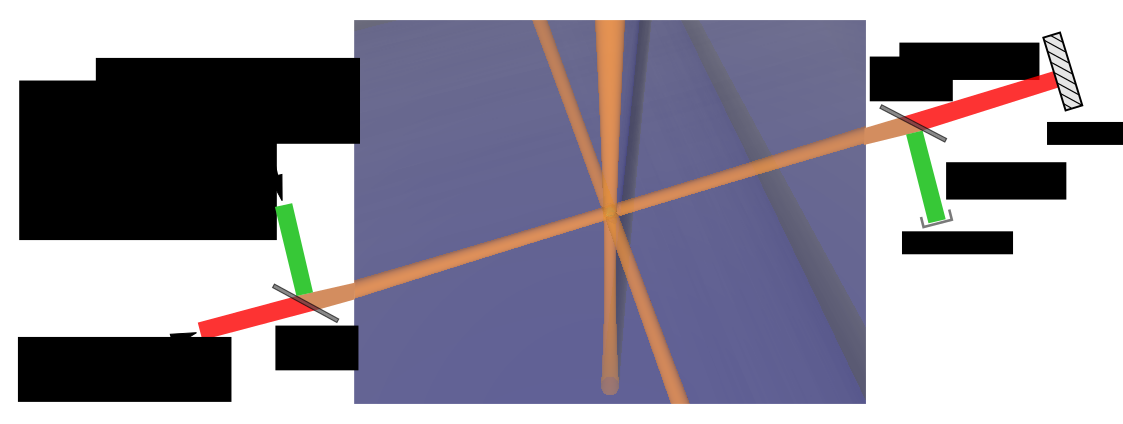
\includegraphics[width=0.8\textwidth]{../figures/lda_evap/compensated_lattice_simple_schematic.png}
\caption{\small Simplified schematic of the compensated lattice setup along one of the
axes.}\label{fig:compensated_lattice_simple_schematic}
\end{figure}

The lattice beam that propagates along the $x$ axis produces a potential of the
form 
\begin{equation}
  V_{L}( x; y,z)  = 
  - s_{0} \exp\left[- 2 \frac{ y^{2} + z^{2} }{w_{L}^{2}} \right]
  \cos^{2}( k_{L} x ) 
\end{equation}
where $s_{0}$ is the lattice depth at the center of the potential,  $w_{L}$ is
the lattice beam waist and $k_{L} = 2\pi/\lambda_{L}$ is the wavenumber of the
lattice light.
The compensation beam that propagates along $x$ produces a potential  
\begin{equation}
  V_{C}( x; y, z)  = 
   g_{0}  \exp\left[ -2 \frac{ y^{2} + z^{2} }{w_{C}^{2}} \right] 
\label{eq:Vcomp}
\end{equation}
where  $g_{0}$ is the depth (or rather height since it is repulsive) of the
compensating potential, and $w_{C}$ is the beam waist of the compensation beam.

The combined potential of lattice plus compensation for the beams propagating
along $x$ is 
\begin{equation}
  V_{1D}( x; y ,z ) = V_{L}(x; y,z) + V_{C}(x; y, z)
\end{equation}

The total potential for our simple cubic lattice is given by 
\begin{equation}
  V_{3D}(x, y, z)  =  V_{1D}( x; y,z) + V_{1D}( y; z,x) + V_{1D}(z; x,y)
\end{equation}


\section{General aspects}
\label{sec:general_aspects}

%In what follows we will first look at general aspects of the potential, using
%analytic approximations to its shape and considering a zero temperature sample.
%Then we will use the high-temperature series expansion (HTSE)\footnote{ The
%HTSE is  an analytical solution to the Hubbard model that is valid at
%high-temperatures.  The HTSE is very good for $T \gg t$ and works down to $T/t
%\sim 1.8$.  This solution gives us the thermodynamic quantities (density,
%double occupancy, entropy per particle, etc.)  for a homogeneous system.}  and
%the local density approximation (LDA) to study the system in more detail. 

Before we go ahead and deploy the full machinery of the LDA+HTSE we will
discuss some general aspects of the potential using analytical approximations
to its shape and considering a zero temperature sample.  We will find that at a
certain ratio of the lattice to compensation beam waist,    $\awaist \equiv
w_{L}/w_{C}$,  one can create a potential optimal for evaporative cooling,
which is also flat at the bottom, in a way reminiscent of the idealized
square-well potential. We will also make an estimate of the atom number
required to realize this setup.

One of the important things to note, is that at each point in space  we will, in
general, have three different lattice depths, associated with each of the
$x,y,$ and $z$ lattice directions. We denote the lattice depths as $s_{x}$,
$s_{y}$ and $s_{z}$, all of which depend on position. To make things simpler,
we can consider the potential along the 111 direction; along this direction
we have equal lattice depths in $x,y,$ and $z$:
\begin{equation} 
  s_{x}( \rdiag ) = s_{y}( \rdiag ) = s_{z}( \rdiag ) = 
  s_{0} \exp \left[ - \frac{ 4 \rdiag^{2} }{3 w_{L}^{2} } \right]  
  \equiv s(\rdiag) 
\end{equation}
where $\rdiag$ represents the distance along the 111 direction.

The bottom envelope of the lattice potential along 111 is given by 
\begin{equation}
  V_{L,\text{env}}( \rdiag )  = -3 s_{0} 
  \exp \left[ - \frac{ 4 \rdiag^{2} }{3 w_{L}^{2} } \right]  
\end{equation}
At each point in space there is a local band structure determined by
$V_{L,\text{env}}$, $s_{x}$, $s_{y}$, and $s_{z}$.  The lowest energy of the
band, which we will refer to  as $E_{0}$, can be approximated by the zero-point
energy of the 3D harmonic oscillator obtained by Taylor expanding the potential
at a lattice site.   This approximation is only valid for deep
lattices\footnote{Recall that the recoil energy, $E_{r}$, is defined as
$\frac{h^{2}}{8m\lambda^{2}}$, where $m$ is the mass of an atom and $\lambda$
is the wavelength of the lattice. } (refer back to 
Fig.~\ref{fig:bands1d} for reference) but we will use it here for its simplicity: 
\begin{equation} E_{0} =  V_{L,\text{env}} +  
     \frac{3}{2} \hbar \omega_{0}  = V_{L,\text{env}} +  3E_{r}\sqrt{ s/E_{r} }. 
\end{equation} 
We can also obtain an expression for the bandwidth, $W$, of the lowest energy
band valid in the limit of deep lattices (cf. Eq.~\ref{eq:tunnelMathieu} or
Ref.~\cite{Bloch2008}):
\begin{equation}
  W =   12 t 
  = E_{r}\frac{48}{\sqrt{\pi}} (s/E_{r})^{3/4} e^{-2\sqrt{s/E_{r}}} .
\end{equation}
Notice that the quantities $E_{0}$, $W$, $\omega_{0}$, $s$, and $t$ are all
position dependent, and thus functions of $\rdiag$. The profiles of these
quantities (and also of the energy of the first excited band, $E_{1}$) are
shown in Fig.~\ref{fig:lattice_general} for a simple cubic lattice  with
lattice beam waist $w_{L}=47\,\mu$m.  

Notice that the Gaussian profile of the lattice beams, being comparable to the
size of typical samples $\approx 40\,\mu$m,  will provide a significant overall
confinement for the atoms. This is in contrast with traditional setups, where
the lattice beam waist is typically larger than 150~$\mu$m and in the length
scale of typical samples the inhomogeneity of the lattice potential is not
noticeable. 
\begin{figure}
    \centering
\includegraphics[width=0.9\textwidth]{../figures/lda_evap/lattice_general.png}
\caption{\small Profiles along $\rdiag$ for a 7$E_{r}$ lattice with
$w_{L}=47\,\mu$m and $\lambda=1064$\,nm.  The energy levels in the lowest band
of the lattice correspond to the shaded blue region.  The curvature of $E_{0}$
determines the confinement.  }
\label{fig:lattice_general}
\end{figure}


\subsubsection{Compensation}
\label{subsec:compensation}

If the lattice beam waist is comparable to the size of the system (as is the
case in our setup),  the confinement from the lattice itself will bee too
large, and it will result in a very large density\footnote{Since we consider
the single band Hubbard model, the density will be saturated at 2 particles per
lattice site.}.  Repulsive compensation beams are then used  to set the
exact amount of confinement in the system and tune its density. 

Beyond simply tuning the density, one can choose a ratio of lattice to
compensation beam waist, defined as $\awaist = w_{L}/w_{C}$~\cite{Mathy2012},
in order to affect the exact spatial dependence of the lowest band.   A setup
which flattens the profile of the lowest band at the center of the trap can
enlarge the size of a local phase which may exist there, an idea suggested in
Ref.~\cite{Mathy2012}, which is at the heart of our compensated lattice design.
In our implementation with Gaussian beams, the lowest band can be made quartic
at best.  This situation may be ideal, because the flat central part of the
lowest band enlarges the extent of the local phase in the center, and the walls
of the potential are not to steep, which lessens the requirements on the
precision of the atom number required to realize a given phase~\cite{Ma2008}.
Besides flattening the band, the use of compensation enables the possibility of
evaporative cooling the sample in the lattice, as we will explain later on.  


\subsubsection{Power series expansion of the lowest band} With the addition of
repulsive compensation beams (depth $g_{0}$ and beam waist $w_{C}$, as in
Eq.~\ref{eq:Vcomp})  we can expand the lowest band profile of the lattice in a
power series as  
\begin{multline} 
  E_{0}(\rdiag)    \approx   
  3( g_{0} + E_{r}\sqrt{s_{0}/E_{r}} - s_{0} )   
  + \left[ 
    \frac{ 4s_{0} - 2E_{r}\sqrt{s_{0}/E_{r}} }{w_{L}^{2} } 
   - 
  \frac{ 4 g_{0} }{ w_{C}^{2}} \right]
  \rdiag^{2}  \\ 
  +  \left[  \frac{ - 8 s_{0} + 2E_{r}\sqrt{s_{0}/E_{r}} }{3 w_{L}^{4} } + 
    \frac{ 8 g_{0} }{3 w_{C}^{4} }  \right] \rdiag^{4}   + 
  \mathcal{O}( \rdiag^{6} )
\label{eq:series_expansion} 
\end{multline}  

If our interest is to maximally flatten the profile of the lowest band, the
quadratic term in the series expansion can be nulled out if one chooses
\begin{equation}
 g_{0} = \frac{  4 s_{0} - 2 E_{r}\sqrt{s_{0}/E_{r}} }{ 4 \awaist^{2} }  
  \equiv g_{\text{quartic}} . 
\end{equation}
If an AFM phase forms at the center of the trap, this
choice of $g_{0}$ will be the most favorable to enlarge the size of the AFM
domain. 

If $\awaist > 1$ and we use a compensation larger than $g_{\text{quartic}}$,
the band profile will have a bump in the center.  Experimentally we have
observed that in that case it becomes hard to align the compensation beams such
that the sample actually stays at the center of the trap.

In our current experiments we use $s_{0}=7\,E_{r}$, and the beam waists in
our setup are calibrated (see Appendix~\ref{app:lattice} for details about the
calibration procedure) to be approximately $w_{L}=47\,\mu$m and
$w_{C}=40\,\mu$m, which gives $\awaist=1.17$.  The necessary compensation to
flatten the band, according to this simplified analytical model, is then
$g_{\text{quartic}} =  4.1\,E_{r}$.


\subsubsection{Evaporation} 

We want to consider the possibility of evaporative cooling in a sample that has
$n=1$ at the center (as is the case for an AFM Mott insulator).   The density
of the sample determines its Fermi energy and, if the Fermi energy is close to
the energy required to escape the potential, evaporation will be effective.
Here, we will consider a cloud with $n=1$ and will set its Fermi energy to
match the energy threshold for evaporation.   This will determine the
compensation $g_{0}$ required for optimal evaporation.   We then equate this
$g_{0}$ with $g_{\mathrm{quartic}}$, obtained above, to find out the parameters
for a trap that is optimal for evaporation and has a flattened bottom. 

To impose $n=1$ at the center we set the global chemical potential\footnote{At
zero temperature the global chemical potential is equal to the Fermi energy.}
to 
\begin{equation}
  \mu_{\text{global}} \equiv \mu(r_{111}=0) = E_{0}(r_{111}=0) + U/2, 
\end{equation}
 where $U$ is the on-site interaction strength \footnote{ For a discussion of
the thermodynamic properties of the Hubbard model refer to
Chapter~\ref{chap:hubbardmodel}} 
%\footnote{ $n(\mu=\bar{E} + U/2)=1$,  is a property of the Hubbard model valid
%at any temperature,  see Fig.~\ref{fig:HTSEhomogeneousA}.  Notice that we are
%measuring the chemical potential with respect to the zero of the optical
%dipole potential.   In the homogeneous Hubbard model $\mu$ is measured with
%respect to $\bar{E}$, and a more familiar expression is $n(\mu=U/2)=1$ (see
%the discussion after Eq.~\ref{eq:hubbard_not_shifted}).  Also, we have
%approximated $\bar{E}\approx E_{0}$ which is valid if the band is narrow, $W
%<< \bar{E}$.} 

At zero temperature, $\mu_{\text{global}}$  can be obtained as the value of
$E_{0}$ at the edge of a cloud that has a a density $n=1$ throughout.  If the
radius of this this half-filled cloud is defined as $r_{\text{hf}}$, the $n=1$
condition can be written as 
\begin{equation}
    \mu_{\text{global}} =  E_{0}(r_{\text{hf}}) = U/2 +  E_{0}(0) 
  \label{eq:half-filling-radius} 
\end{equation} 
This situation is illustrated in Fig.~\ref{fig:lattice_general-comp} (see right
panel).  
\begin{figure}
    \centering
\includegraphics[width=1.0\textwidth]{../figures/lda_evap/lattice_general-comp.png}
\caption{\small Profiles along $\rdiag$ for a 7\,$E_{r}$ lattice with
$w_{L}=47\,\mu$m.  The chemical potential is set to match the threshold for
evaporation, and the compensation is set to $g_{0}=g_{\text{quartic}}$. This
conditions determine the waist ratio $\awaistevap$ (see text).  The panel on
the right shows the energy of the band close up, and the panel of the left is
zoomed out to reveal the small scale of the band energies compared to the
energies of the optical dipole potential. }
\label{fig:lattice_general-comp}
\end{figure}

For optimal evaporation in the trap we need $\mu_{\mathrm{global}}$ to come as
close as possible to the evaporation threshold energy, $E_{\text{th}}$.  In our
setup, $E_{\text{th}}$ is the energy required to escape along one of the
lattice beams\footnote{Since we have set the zero of energy at infinity (where
no dipole potentials exist), the energy threshold to escape along a beam is
negative.}: 
\begin{equation} 
  E_{\text{th}} =  -s_{0} + E_{r}\sqrt{s_{0}/E_{r}} + g_{0}  \equiv E_{0}(0)/3 
\end{equation}

Setting $\mu_{\text{global}} = E_{\text{th}} $.
This condition, along with Eq.~\ref{eq:half-filling-radius}, results in
\begin{equation}
   U/2 + E_{0}(0) =  E_{0}(0)/3
   \ \ \ \  \Rightarrow \ \ \ \ 
    \frac{U}{2} = -\frac{2}{3} E_{0}(0)  
   \ \ \ \  \Rightarrow \ \ \ \  
   g_{0} =  -U/4  + s_{0} -  E_{r}\sqrt{s_{0}/E_{r}}
%  -2( g_{0} + E_{r}\sqrt{s_{0}/E_{r}} - s_{0} ) = U/2  
  \label{eq:optimal-evap} 
\end{equation} 

We recall that  $g_{\text{quartic}} = \frac{  4 s_{0} - 2
E_{r}\sqrt{s_{0}/E_{r}} }{ 4 \awaist^{2} } $. From Eq.~\ref{eq:optimal-evap} we
obtain the equation that defines $\awaistevap$,  the beam waist ratio that
optimizes evaporation while flattening the bottom of the band: 
\begin{equation}  
   \frac{  4 s_{0} - 2 E_{r}\sqrt{s_{0}/E_{r}} }{ 4 \awaist^{2} }  
   =  -U/4  + s_{0} -  E_{r}\sqrt{s_{0}/E_{r}}
\end{equation} 
Solving we obtain:
\begin{equation}
 \awaistevap^{2} =  \frac{ 4 s_{0} - 2 E_{r} \sqrt{s_{0}/E_{r} }}
    { 4s_{0} - 4 E_{r} \sqrt{s_{0}/E_{r}}  - U } 
 \label{eq:awaistevap}  
\end{equation} 
\begin{figure}
    \centering
\includegraphics[width=0.7\textwidth]{../figures/lda_evap/alpha-evap-optimal.png}
\caption{\small Optimal beam waist ratio for enlarging the central flat portion on
the band and maximizing the rate of evaporative cooling. }
\label{fig:alpha-evap-optimal}
\end{figure}
In Fig.~\ref{fig:alpha-evap-optimal} we show plots of $\awaistevap$ for various
values of $U/t$ as a function of lattice depth.  For a 7\,$E_{r}$ lattice
$\awaistevap$ is between 1.14 and 1.20, depending on the interaction strength.  

We conclude from the analytical considerations presented in this section that, for a
$7\,E_{r}$ compensated lattice,  a  beam waist ratio $\awaist \approx 1.17$ and
compensation $g_{0}=g_{\text{quartic}}$ will offer the best scenario for
evaporation while flattening the bottom of the band.  


%For a deep lattice ($\gtrsim 10\,E_{r}$) the on-site interactions can be
%expressed analytically as \begin{equation} \frac{U}{E_{r}}  =  4 \sqrt{2\pi}
%\frac{ a_{s} }{\lambda}  (s/E_{r})^{3/4} \label{eq:onsite-analytic}
%\end{equation} The scattering length is usually expressed in units of the Bohr
%radius, $a_{0}$, so it is useful to keep in mind that for our 1064~nm lattice
%$\lambda = 20113\ a_{0}$.  In our experiment we want to avoid very large
%scattering lengths because they give rise to fast inelastic losses that scale
%as $a_{s}^{4}$; reasonable values of $a_{s}$ are up to 800\,$a_{0}$.   In a
%7\,$E_{r}$ lattice a scattering length $a_{s}=800\,a_{0}$ implies an
%interaction strength $U/t=35$, calculated from Eq.~\ref{eq:onsite-analytic}.


\subsubsection{Atom number}
 
We now turn to examine the number of atoms required to realize the setup
described above.  We need to solve for the half-filling radius,
$r_{\text{hf}}$, which is defined by Eq.~\ref{eq:half-filling-radius} (and also
graphically on the right panel of Fig.~\ref{fig:lattice_general-comp}).  Using
$n=1/a^{3}$, where $a$ is the lattice spacing, we obtain the atom number
from the radius, as $N_{\text{hf}} = \frac{4}{3} \pi (r_{\text{hf}}/a)^{3}$.  

To solve for $r_{\text{hf}}$ we can use the power series expansion of the band
energy (Eq.~\ref{eq:series_expansion}), which for $g_{0}=g_{\text{quartic}}$ is 
\begin{equation}
  E_{0}(r_{\text{hf}}) - E_{0}(0) = \left[  
  \frac{  2E_{r}\sqrt{s_{0}/E_{r}} - 8s_{0} 
   + 4( 2s_{0} -E_{r}\sqrt{s_{0}/E_{r}} ) \awaist^{4} }
  { 3 w_{L}^{4} } \right] r_{\text{hf}}^{4} =  \frac{U}{2}  
\end{equation}
The solution for $r_{\text{hf}}$ is then 
\begin{equation}
  r_{\text{hf}} =  \frac{w_{L}}{\awaist} \left[ 
  \frac{3}{2}  
  \frac{( 1 - 2\awaist^{4} + 2 \sqrt{s_{0}/E_{r}}( \awaist^{4} -1 ) )}
  { ( 1 -  2\awaist^{4} + 4 \sqrt{s0/E_{r}} ( \awaist^{4} -1 ) ) } 
  \right]^{1/4} 
\end{equation}
For $s_{0}=7,E_{r}$ and $\awaist=1.17$,  $r_{\text{hf}}\approx 0.7 w_{L}$.  For
a lattice beam waist $w_{L}=47\,\mu$m  this amounts to $N_{\text{hf}}=990,000$
atoms.    

%When using compensation we will find that we can use smaller beam waists and
%that the potential has the capacity to accommodate a larger number of atoms.
%Since the size of the sample starts becoming comparable to the lattice beam
%waist, we can no longer work in the harmonic approximation.   In later
%sections we will turn to the more precise implementation of the local
%density approximation, and we will calculate the relevant local quantities
%($U$, $t$, etc. ) numerically, without making any deep lattice or harmonic
%approximations. 
% 


\subsubsection{Current setup} 

In our current setup we use a lattice depth $s_{0}=7\,E_{r}$, and we have
approximately $w_{L}=47\,\mu$m and $w_{C}=40\,\mu$m,  which corresponds to
$\awaist=1.175$.   As we have seen above, we should compensate this sample with
$g_{\text{quartic}} = 4.11\,E_{r}$ and populate it with $N\approx 990,000$
atoms.  This would yield a sample with $n\approx1$ at the center, and a
potential with optimal conditions for evaporative cooling in the lattice.   

Empirically, we have found that with $N=200,000$ atoms we obtain the largest
amount of AFM correlations, as measured by Bragg scattering of light (see
Chapter~\ref{chap:afmbragg}).  With this number of atoms, the compensation has
to be reduced down to $3.6\,E_{r}$ to obtain a density $n\approx1$ at the
center (see Appendix~\ref{app:lattice} for more details on the calibration of
the compensation).  Reducing the atom number and the compensation moves us away
from the optimal scenario for evaporative cooling in the lattice. 

There are two other important factors that play a role in our ability to detect
AFM correlations.  The first one has to do with the stability of our setup and
the ability to make a reproducible potential.   It turns out that when the
optimal value of compensation is used, slight drifts in the alignment of one of
the lattice or compensation beams have a strong effect on the density
distribution of the cloud.  This presents problems when taking data because one
cannot reliably realize comparable samples.  

The second factor has to do with our measurement procedure.   We measure AFM
correlations by using Bragg scattering of light.  Before probing the system we
project its state onto a product state where each lattice site is isolated from
the rest and has a well defined occupation.  This is done by quickly ramping up
the power of the lattice beams to change the lattice depth from $7\,E_{r}$ to
20$\,E_{r}$.   This achieves the desired projection and freezes any tunneling
between neighboring sites.  If the atoms occupy a large fraction of the lattice
beam waist (the optimal setup described above requires
$r_{\mathrm{hf}}=0.7w_{L}$), the lattice lock to 20\,$E_{r}$ can have a
negative effect on the sample, preventing us from observing the AFM
correlations.  We will elaborate more on this point in \S~\ref{subsec:locking}.

%Unfortunately we only have $\approx$200,000 atoms at our disposal at this stage
%of the experiment (see Chapter~\ref{chap:expsetup}).   In practice, this forces
%us to reduce the compensation below $g_{\text{quartic}}$  so that we can
%achieve $n=1$ at the center.   Reducing  the compensation significantly reduces
%the efficiency of evaporative cooling in the lattice, but we have no choice
%because we must have $n=1$ at the center to realize the AFM Mott insulating
%phase that is of most interest to us. 
%
%The value of $N=200,000$ was found empirically to be where the strongest Bragg
%signals were observed.   We can load more atoms into the lattice and use a
%larger compensation to obtain $n=1$, but our Bragg scattering signal starts
%getting weaker.   In principle, with more atoms and more compensation the Bragg
%signal should be stronger because the extent of the Mott plateau would be
%enlarged.  However, we do not see this in the experiment.   We see better signals
%for low atom numbers and less green.   
%
%Prior to shining the Bragg probe we ramp
%up the lattice up to 20\,$E_{r}$ to freeze  tunneling and enhance the
%Debye-Waller factor. We suspect that the lattice locking ramp may be related to
%why we get the best signals with low atom number.  For a fixed number of
%atoms we also found that using larger lattice depths for the lock would
%deteriorate the Bragg scattering signal. 
 
%\paragraph{Why is our atom number 300,000?}   At the moment our
%experimental sequence consists of the following steps:
%\begin{enumerate}
%\item  Evaporate into a dimple potential with a depth of $\approx 0.5\,E_{r}$
%per axis.   The cold sample in the dimple has a density of nearly one atom
%per site.  
%
%\item  Rotate the polarization of the retro beams to go from dimple to lattice
%configuration.   We want the sample in the dimple to have a Fermi energy $E_{F}
%< E_{r}$ so that we can be sure that all of the atoms will remain in the lowest
%band  as we rotate to a lattice potential.   While we rotate we add a minimal
%amount of compensation, 0.06\,$E_{r}$.  
%
%\item  Ramp up the lattice depth in 25 ms up to the point where the lowest band
%and first excited band separate, which corresponds to a lattice depth of
%$\approx 2.4\,E_{r}$.  At the same time add 0.65\,$E_{r}$ of compensation.
%During this time also ramp the interaction strength from the evaporation value
%to the value we want in the experiment.  
%
%\item Ramp up, in 15 ms,  the lattice depth to 7\,$E_{r}$ and the compensation
%to the desired final value.
%\end{enumerate}
%
%So far in our experiments we have tried to keep the density at one per site
%from the moment we start in the dimple at Step 1, up to the final sample in
%the lattice.    Keeping the density at $n=1$ gives us a constraint for the
%number of atoms that we start with in the dimple potential.   We derive this
%below. 
%
%In the dimple, having a peak density of one per site translates into having a
%global trap Fermi energy which is $E_{F,\text{trap}} \approx E_{r}$.   The
%local Fermi energy and the density at the center of the trap can be related by
%$E_{F} = \frac{\hbar}{2m} ( 3\pi^{2} n)^{2/3}$.  Setting the density to one per
%site, $n=a^{-3}$ yields  $E_{F} = (3/\pi)^{2/3} E_{r} \approx 0.97 E_{r}$.
%The local Fermi energy at the center will be the same as the global Fermi
%energy of the harmonic trap, so we can find the total trapped atom number from 
%\begin{equation}
%  E_{F,\text{trap}} = \hbar \omega ( 3 N )^{1/3}  = E_{r}  
% \ \ \ \  \Rightarrow  \ \ \ \  N = \frac{1}{3} 
%  \left( \frac{ E_{r}} {\hbar \omega} \right)^{3} 
%\end{equation} 
%
%A dimple potential with depth $V_{0}$ per axis has a trapping frequency 
%\begin{equation}
%  \omega  =  \left( \frac{8V_{0} } { mw_{L}^{2} } \right)^{1/2}
%  =   \frac{ a \sqrt{2E_{r}} }{ \hbar \pi} 
%   \left(  \frac{8V_{0} } { w_{L}^{2} } \right)^{1/2}
%  =   \frac{ 4 a  }{ \hbar \pi w_{L} } 
%   \left(  E_{r}V_{0}  \right)^{1/2}
%\end{equation} 
%so 
%\begin{equation} 
% N = \frac{1}{3} 
%  \left(  \frac{ \pi w_{L} }{ 4a} \right)^{3}  
%  \left( \frac{ E_{r} }{V_{0}} \right)^{3/2} 
%\end{equation}
%With $V_{0} = 0.5\,E_{r}$ and $w_{L}=47\,\mu$m we obtain $N = 315,000$ atoms. 
%
%Just notice that for this calculation to make sense, the depth of the dimple
%potential has to be larger than the Fermi energy in the harmonic trap, that is 
%\begin{equation}
%  2 V_{0} >  E_{F,\text{trap}}
%\end{equation} 
%In our setup we just match this condition since $2V_{0}= 1\,E_{r}$ and
%$E_{F,\text{trap}} = 1\,E_{r}$.  
% 
%\paragraph{Can we load more atoms into the lattice?}  In order to load more
%atoms into the lattice we would have to start with a larger number of atoms in
%the dimple.  If we were to initially load a deeper dimple then, for our beam
%waists, the sample would have a density larger than one per site at the center.
%This poses a problem because the Fermi energy would be larger than 1\,$E_{r}$,
%and it would lead to population of the first excited band when rotating into
%the lattice.  Furthermore we do not know if we can achieve as low
%temperatures as we do in the 0.5~\,$E_{r}$ dimple.   
%
%A simple way to circumvent the higher band issue would be to compensate the
%dimple before rotating the polarization of the retro beams.  In that way, a
%larger atom number can be accommodated at a density of one atom per site, and we
%could proceed with the ramps that maintain the density at that value.  With a
%larger atom number we would find that we would require a larger $g_{0}$, closer
%to $g_{\text{quartic}}$, in order to get to half-filling in the final sample.  
%
%
%\paragraph{Why do we stick with 300,000 atoms?}  We go back to the first
%consideration of this section:  locking the lattice.   If we load a sample of
%more than $N=230,000$ atoms the lattice lock to 20\,$E_{r}$ compromises our
%measurement by forcing atoms into the first excited band.   Already at our atom
%number of $N\approx 300,000$ the lock to 20\,$E_{r}$ poses somewhat of a
%compromise.
%
%\paragraph{Considerations for future improvements.}  The main bottleneck for
%our setup at the moment is related to the lock.  A lattice beam waist of
%$w_{L}=70\,\mu$m  would allow us to lock up to 35\,$E_{r}$ with a sample of
%$N=300,000$ atoms.   
%
%In the next section we will use the quantitative results of the LDA to gain
%more insight into the compensated lattice setup and help us decide on the best
%parameters for the future improvements of our setup.



\section{ Local density approximation }
\label{sec:lda}

In what follows we will investigate in more detail the properties of the
compensated lattice setup using the LDA+HTSE.   In the local density
approximation (LDA), we consider each point in the potential as a homogeneous
system and we set the condition that all of these local homogeneous systems are
in thermal equilibrium with each other  at some temperature $T$.   At each
point in space we can obtain a local value of the lattice depth, which along
with the scattering length, determines the local values of the Hubbard
parameters $t$ and $U$.  With these in hand, we can use a known solution to the
homogeneous Hubbard model (the HTSE) and obtain local values for the
thermodynamic quantities, such as density, double occupancy, entropy, etc.   We
can then plot the local thermodynamic quantities as a function of trap position
to obtain trap profiles.  

\subsection{Format for presentation of LDA results} 

\begin{figure}
    \centering
\includegraphics[width=0.75\textwidth]{../figures/lda_evap/figures_hubbard-lda/005.png}
\caption{\small Red detuned uniform lattice with additional harmonic confinement.  The
confinement is adjusted so that the density is one per site at the center with
$N=300,000$ atoms.   The temperature is set to $T=0.12\,E_{r}$, which results
in an overall entropy per particle  $S/N=1.63k_{\text{B}}$. See the text for a
detailed explanation of the information in this plot.}  
      \label{fig:HTSE_LDA_harmonic}
\end{figure}
 
An example of the results that are obtained within the LDA is shown in
Fig.~\ref{fig:HTSE_LDA_harmonic} for a (nearly) uniform lattice potential plus
harmonic confinement, i.e. a traditional lattice setup.  Notice that to obtain
the uniform lattice plus confinement we use the geometry of our current setup
(parameters are $s_{0},g_{0}, w_{L}, w_{C}$), but we set large values of the
beam waists for the lattice and compensation beams, and set a negative depth
($g_{0}<0$) for the compensation.  
%The resulting trap frequencies in this setup are $\bar{\nu} =
%352\,\mathrm{Hz}$ in all three directions, calculated for $^{6}$Li. 

In Fig.~\ref{fig:HTSE_LDA_harmonic} the large panel shows the
relevant energies as a function of distance (in $\mu$m) along the 111 body
diagonal of the lattice.   The small panel shows the corresponding profiles of
the thermodynamic quantities calculated with the LDA+HTSE. We now give detailed
information about each of the labels and regions displayed in
Fig.~\ref{fig:HTSE_LDA_harmonic}.

\paragraph{Energies and figures of merit for evaporation} 

\begin{itemize} 

\item \textbf{Parameters of the potential.}  The labels on the top left indicate
the depth of the lattice and compensating potentials in recoils, and also the
waists used for the lattice and compensating beams.   Also
shown are the beam waist ratio, $\awaist$ and the confinement frequency
$\bar{\nu}$, which is calculated from the curvature of the bottom of the lowest
band at the center.  At the top left we also show values for $\eta_{F}$ and
$\Delta_{F}$.  The meaning of these quantities will be explained below. 

\item \textbf{Hubbard parameters.}  The labels on the top right of the main
plot indicate the scattering length and the resulting Hubbard parameters for
the given the lattice depth.  The values of $U/t$, $T/t$, and $t$ given are
for the center of the sample.  As one moves away from the center, $t$
increases and  $U/t$ and $T/t$ decrease.
 
\item \textbf{Lattice potential} (gray line). This line shows a representation of the
modulation produced by the lattice potential.   The period of the modulations
shown is arbitrary and for illustration purposes only.  A thin line is also
plotted showing the envelope of the lattice potential.  



\item \textbf{Band lower half} (blue shaded region).  This is the blue shaded
region on the large panel. The bottom line corresponds to the lowest energy
level accessible to a single particle in the local  Hubbard Hamiltonian.   The
top line corresponds to the energy at the center of the lowest band.   

The central energy of the lowest band is an important reference in the Hubbard
model, as we saw in Chapter~\ref{chap:atomsinlattices}.    The Hamiltonian for a single particle in a lattice is  
\begin{equation} 
  H  = -\frac{\hbar^{2}}{2m} \frac{ \partial }{ \partial x^{2} } +  
       V_{0} \sin^{2}(kx)  
\end{equation}  
where the zero of energy is at the bottom of a lattice site.  The energy level
structure as a function of lattice depth is as shown in
Fig~\ref{fig:Hubbard-firstquant}.   In second quantized form this single
particle Hamiltonian is usually written as  
\begin{equation} 
  H  = -t \sum_{ \langle ij \rangle, \sigma } a_{i\sigma}^{\dagger} a_{j\sigma} 
  \label{eq:Hubbard-free-secondquant}
\end{equation}  
What is typically not mentioned is that writing the Hamiltonian as in
Eq.~\ref{eq:Hubbard-free-secondquant} implies a lattice-depth-dependent  shift
of the energy zero, such that the band structure looks like in
Fig.~\ref{fig:Hubbard-secondquant} (see also the discussion after
Eq.~\ref{eq:hubbard_not_shifted}).  In Chapter~\ref{chap:hubbardmodel}, when
solving the Hubbard model using the HTSE, we used the second quantized form of
the Hamiltonian, so the chemical potential is referenced from the center of the
lowest band.    
\begin{figure}
        \centering
        \begin{subfigure}[t]{0.4\textwidth}
		\includegraphics[width=\textwidth]{../figures/lda_evap/bands1d_V0_firstquant.png}
\caption{\small Band structure when the zero of energy is at the bottom of the
lattice sites.  The zero of energy does not change with lattice depth, and the
band energies go up almost like the harmonic oscillator state in an individual
lattice site.  }
                \label{fig:Hubbard-firstquant}
        \end{subfigure}%
        ~~ %add desired spacing between images, e. g. ~, \quad, \qquad etc.
          %(or a blank line to force the subfigure onto a new line)
        \begin{subfigure}[t]{0.4\textwidth}
		\includegraphics[width=\textwidth]{../figures/lda_evap/bands1d_V0_secondquant.png}
\caption{\small Band structure when the zero of energy is at the center of the lowest
band.  This shift is implicit when the Hamiltonian is written in second
quantized form as in Eq.~\ref{eq:Hubbard-free-secondquant}.  }
                \label{fig:Hubbard-secondquant}
        \end{subfigure}
	\caption{\small Band structure in the Hubbard model.  }
\label{fig:Hubbard-first-second}
\end{figure}

Most importantly, the average energy of the lowest band is a ubiquitous energy
in the Hubbard model because states below that energy will be almost
unperturbed by interactions, whereas states above that energy will be affected
significantly by interactions (cf. the exact diagonalization eigenvalues for a
double-well and a plaquette show in Figs.~\ref{fig:exact_2site}
and~\ref{fig:exact_4site}). 

\item \textbf{Band upper half + $\mathbf{U}$ } (purple shaded region)  This
region represents the energy levels in the upper half of the lowest band
shifted up by the interaction, $U$.  This simple picture is not correct in the
interacting many-body system but it provides a good representation of what is
going on.  The separation $U$ between the band lower half and the band upper
half represents the Mott-Hubbard gap. 


\item \textbf{First excited band} (red region).   This region is simply bounded
by the lowest and highest energies in the first excited band.  For this band we
do not apply shifts due to interactions.   This band is shown so that, at a
glance, one can asses whether or not the system satisfies the single band
Hubbard regime (see Fig.~\ref{fig:hubbardvalid}).  

\item \textbf{Global chemical potential} (green line).  A fixed global
chemical potential is set across the cloud.  The local chemical potential is
obtained by looking at the separation between $\mu_{0}$ and the local zero of
energy.   We remind the reader that the local zero of energy is the point at
the center of the lowest band, i.e. the upper boundary of the blue shaded
region.

\item \textbf{Evaporation threshold} (orange line).   This is the energy
required to escape along one of the lattice beams.  It is calculated by looking
at the profile of the lowest energy level along the 100 direction and finding
its maximum.    In most cases the maximum will be at infinity, but for $\awaist
< 1 $ the lowest band profile along 100 can have a local maximum.   In such
cases the local maximum is used as the evaporation threshold, since an atom has
to exceed that energy to escape the trap.  


\item \textbf{Figures of merit for evaporative cooling in the lattice
($\eta_{F},\ \Delta_{F}$).} 

When evaporative cooling a thermal gas of atoms, one considers the parameter
$\eta=U_{\text{trap}}/\kb T$, where $T$ is the temperature of the gas, and
$U_{\text{trap}}$ is the energy threshold required for a particle to leave the
trap  measured with respect to the lowest single-particle
energy state.  The evaporation rate is suppressed by a factor $\exp(-\eta)$
where typically $\eta\sim10$ for efficient evaporation,  and, as the gas cools
down, the trap depth is reduced to force further evaporation~\cite{OHara2001PRAb}.  

For a deeply degenerate Fermi gas ($T \ll T_{F}$, where $T_{F}$ is the Fermi
temperature) the evaporation rate is given by~\cite{OHara2001PRAb}.
\begin{equation}
  \Gamma_{\text{evap}} \propto \gamma_{\text{coll}} \frac{T}{T_{F}} 
  \exp\left[ -   
  \frac{ U_{\text{trap}} - \kb T_{F} }{ \kb T }  \right ] 
\end{equation}
where $\gamma_{\text{coll}}$ is the classical collision rate evaluated at the
Fermi surface and the exponential factor corresponds to the tail of the
Fermi-Dirac distribution.   At fixed temperature, the evaporation rate
$\Gamma_{\text{evap}}$ will depend only on $U_{\text{trap}} - \kb T_{F}$, which
can be approximated as   $\Delta_{F} = U_{\text{trap}} - \mu_{0}$.   If we
consider fixed entropy\footnote{The entropy of a Fermi gas in a harmonic trap
is given by $S=N\pi^{2} T/T_{F}$~\cite{Kohl2006} for $T\ll T_{F}$.} rather than
fixed temperature, we can write  
\begin{equation}
  \Gamma_{\text{evap}} \propto \gamma_{\text{coll}} \frac{T}{T_{F}}
  \exp\left[ \frac{1}{T/T_{F}} \right]  
  \exp\left[ -  \frac{1}{T/T_{F}} \left( \frac{U_{\text{trap}}}{\kb T_{F}} \right) \right] 
\end{equation}
We define $ \eta_{F} \equiv U_{\text{trap}}/\kb T_{F}$ and observe that 
\begin{equation}
  \Gamma_{\text{evap}} \propto \gamma_{\text{coll}} \frac{T}{T_{F}}
  \exp\left[ -  \frac{\eta_{F} - 1 }{ T/T_{F} } \right]
\end{equation}
For a given value of the entropy ($T/T_{F}$), the rate depends only on
$\eta_{F}$,  and thus the parameter $\eta_{F}$ can serve as a figure of merit
for evaporation. 

In terms of $\Delta_{F}$ or $\eta_{F}$,  the effective factor,
$\eta_{\text{eff}}$, which determines the exponential suppression of
evaporation due to the trap depth is given by
\begin{equation}
 \exp(-\eta_{\text{eff}})  
  =  \frac{T}{T_{F}} \exp \left[ - \frac{ \Delta_{F} }{ \kb T} \right]
  =  \frac{T}{T_{F}} \exp\left[- \frac{\eta_{F} - 1 }{T/T_{F} } \right]
\end{equation}
Besides the Boltzmann exponential suppression, the evaporation rate is
additionally suppressed by a factor $T/T_{F}$ due to Pauli blocking of one of
the final states of a collision, which occurs for $T\ll
T_{F}$~\cite{OHara2001PRAb}.    
%For a value of $T/T_{F}=0.1$ to get
%$\eta_{\text{eff}}=10$ we need $\eta_{F} = 1.77 $ 

\end{itemize}

\paragraph{ Thermodynamic quantities} 

\begin{itemize} 
 
\item \textbf{Trap profiles of thermodynamic quantities.}  The smaller panel on
the top left corner on Fig.~\ref{fig:HTSE_LDA_harmonic} shows the trap profiles
of the thermodynamic quantities.   It includes the density ($n$), double
occupancy ($d$), entropy per lattice site ($s_{L}$) and entropy per particle
($s_{N}$).  The entropy per particle is plotted on the right side axis.

\item \textbf{Overall values of the thermodynamic quantities.} The labels above
the smaller panel in Fig.~\ref{fig:HTSE_LDA_harmonic} indicate the overall trap
values of the thermodynamic quantities: number ($N$), double occupancy ($D$)
and entropy per particle ($S/N$).  These are obtained by integrating the local
values across the volume of the trap.  Also shown is the half-width at half-max
(HWHM) of the density distribution in units of the lattice beam waist.  

\end{itemize}


The LDA results for a given trap, as exemplified by
Fig.~\ref{fig:HTSE_LDA_harmonic}, will serve as the point of comparison for
different trap parameters.  To assess the ability to evaporatively cool in a
given setup we will look at $\eta_{F}$ and $\Delta_{F}$.  Beyond that, the atom
number is important for practical considerations, and as we will now explain,
the resulting overall entropy per particle is an important metric as
well. 


\subsection{ Entropy redistribution }

When considering the possibility of accessing the ground state of the Hubbard
Hamiltonian, the overall entropy per particle, $S/(N\kb)$, is an important
quantity.  It determines the number of quantum states that are accessible to
each atom.  At half-filling there is an average of one-particle per site;  if
the temperature of the system is high, $T\gg U$, there is an equal probability
for a site to be empty ($|0\rangle$), singly ($|\nspup\rangle \ \text{or}\
|\nspdn\rangle$)  or doubly ($|\ndbl\rangle$) occupied.  With four equally
probable states at each lattice site, the entropy per particle\footnote{Notice
that at half-filling any quantity per particle is the same as per lattice site,
since $n=1$}  is $\ln 4 = 1.38$.

When the temperature is $T\ll U$, double occupancies and vacancies are suppressed
and the system enters the Mott insulating state.  At each site, a
particle can still  be spin-up or spin-down with equal probability, so the
entropy per particle becomes $\ln 2 = 0.69 $.   

If the temperature of the system goes below the N\'{e}el temperature, the atoms
start to order antiferromagnetically.  At zero temperature each site has only
one possible quantum state (spin-up or spin-down depending on the lattice site)
and the entropy per particle goes to zero\footnote{Strictly speaking, at $T=0$
the entire system can be in only one of two quantum states corresponding to the
two possible orientations of the antiferromagnet. The entropy per particle is
$\ln2/N$ which goes to zero for very large $N$.}.  

Numerical studies calculate the highest value of the N\'{e}el temperature for a
homogeneous simple cubic lattice to be $0.33t \lesssim T_{N} \lesssim 0.36t$,
occurring at $U/t=8$~\cite{Fuchs2011,Paiva2011,Kozic2013}.   As we have
explained, real systems with a finite number of atoms and external confinement
have an inhomogeneous density profile that decays as a function of distance to
the center.  If one creates an AFM domain at the core of the sample, it will be
surrounded by a shell where $n<1$.   We saw in Chapter~\ref{chap:hubbardmodel}
that the metallic phase at $n<1$ has an enhanced entropy capacity which grows
as $n\rightarrow 0$.  This leads to the concept of entropy redistribution in
the inhomogeneous trap:  the shell will carry the largest fraction of $S/N$,
and this will result in a lower local value of the entropy at the core,
enhancing the possibility of accessing an ordered phase.   In
Ref.~\cite{Paiva2011} it is shown that the N\'{e}el entropy per particle
necessary to achieve an ordered phase, which is $S/(N\kb) \approx 0.36$ for a
homogeneous sample, can be as large as $S/(N\kb) \approx 0.6$ in a harmonically
trapped sample. 

This shows that the presence of the trap, although a deviation from the ideal
model, serves as means to facilitate the realization of ordered phases.   When
considering a particular implementation of the potential, there is a trade-off
between entropy redistribution and flatness of the band.  In the limit of a
square-well confinement there is no entropy redistribution at all, but if
the AFM phase is realized it will occupy the entire trap.   On the other hand
for a harmonic trap entropy redistribution enables the creation of an AFM core
at slightly larger entropies than in the homogeneous case, but the AFM domain
will occupy a small fraction of the sample.  

%For a homogeneous 3D lattice, at the N\'{e}el temperature $T_{N}=0.36t$, the
%entropy per particle is $s=0.4\,\kb$.  As the temperature starts dropping below
%$T_{N}$ the entropy approaches zero very quickly in what is referred to as the
%AFM transition (AFM stands for antiferromagnetic order).  The AFM transition
%has been studied theoretically for homogeneous 3D systems using  quantum
%Monte Carlo (QMC)~\cite{Paiva2011} and the dynamical cluster approximation
%(DCA)~\cite{Fuchs2011}.  The results from these two approaches are shown in
%Figs.~\ref{fig:paiva-entropy3D},\ref{fig:fuchs-entropy3D}.
%
%The theoretical calculations shown correspond to a homogeneous system, but in
%practice  one has samples with a finite number of atoms so one is forced to
%confine them in order to reach half-filling.   Since the confinement is
%typically harmonic (as opposed to a well with hard walls), the density decays
%as a function of distance to the center.   The inhomogeneity in the density
%leads to the concept of entropy redistribution.  As a consequence, the overall
%entropy per particle  necessary to achieve a N\'{e}el state can be higher in a
%trapped system that in the homogeneous case~\cite{Paiva2011}. 


When comparing different trapping potentials, there are two ways to quantify
the amount of entropy redistribution.  One can calculate the trap properties at
a fixed value of $S/N$ and compare the resulting temperature for the different
trap parameters;  the one with the lowest $T$ will be better at entropy
redistribution.   Alternatively, one can do the calculation at fixed $T/t$ and
compare the resulting values of $S/N$.  At fixed $T$ a larger value of $S/N$ is
indicative of better entropy redistribution. 


%\subsection{ Comparing  entropy redistribution scenarios} 
%
%We can consider compensated lattice setups with different beam waist ratios
%$\awaist$ and different compensation values and determine which setup offers
%the best scenario for entropy redistribution.  There are two approaches to do
%this. 
%
%One can realize the LDA at a fixed value of $S/N$, find out the resulting
%temperature of the sample and compare the different scenarios.   Alternatively
%one can realize the LDA at a fixed temperature and compare the values of $S/N$
%for different scenarios.   
%
%The first method is more closely related to experiments, because ultracold
%atoms are isolated systems and the loading of atoms into the lattice should, in
%principle, proceed adiabatically.   In this way one can see for different
%setups how will the system be adiabatically heated or cooled as it is loaded
%into the lattice.   Since the entropy is a monotonic function of the
%temperature,  the approach which realizes the LDA at fixed temperature and
%compares the resulting $S/N$ is also valid.  This approach is easier to
%implement in the computer code, since the solution to the HTSE is obtained from
%the grand canonical partition function, which assumes the system is at fixed
%temperature.  

\section{Results}

After explaining the results that the LDA calculation can offer for a given
trap, and introducing the figures of merit for evaporation and entropy
redistribution,  we will now show results for different values of the beam
waist ratio , $\awaist$.  


We start by considering the evaporation figure of merit.  We set the global
chemical potential such that $n=1$ at the center of the sample and we find the
largest compensation that the setup will tolerate based on the following
constraints:

\begin{myblock}
 \textbf{Constraint 1:} The lowest band is required to have positive
curvature at the origin (avoid Mexican hat type band profile).  Also, the
resulting density profile is required to decrease monotonically as a function
of distance from the center.
\end{myblock}
\vspace{-2em}
 
\begin{myblock}
\textbf{Constraint 2:} The thermal tail of the Fermi distribution is required
to be negligible below the asymptotic energy of an atom along one of the
lattice axes (avoid spilling atoms into the lattice beams).  This condition can
be written as   \[  \mu + T < E_{100}(\infty), \] where $E_{100}(\infty)$ is
the asymptotic bottom of the band along the 100 lattice beam.  
\end{myblock} 
\vspace{-2em} 
\begin{myblock} 
\textbf{Constraint 3:} The thermal tail of the Fermi distribution is required
to be negligible below  the threshold energy for evaporation: \[  \mu + T <
E_{\mathrm{th}} \] 
\end{myblock}

Depending on the value of $\awaist$ one of these three constraints will
determine the largest compensation.  Below we explain the possible scenarios:


\vspace{-1.5em}
\begin{myblock}
  \underline{\textbf{Scenario 1},~~$\awaist = \awaistevap$} \newline This is
the optimal scenario for both band flattening and evaporation. In this case the
curvature of the lowest band at the origin is zero (optimal flattening,
$E_{0}(r_{111})\propto r^{4}$),  and $\mu + T = E_{\text{th}}$ (optimal
evaporation).  Back in Eq.~\ref{eq:awaistevap} we used a zero temperature
analytical model to derive an expression for $\awaistevap$, which we found to
be  $\awaistevap \approx 1.15$ for 7\,$E_{r}$ and $U/t=24.8$
($a_{s}=650\,a_{0}$).
\end{myblock}
 
\vspace{-2em}
\begin{myblock} 
  \underline{\textbf{Scenario 2},~~$ 1 < \awaist < \awaistevap$} \newline
Constraint 3 determines $g_{0}$,  evaporation is optimal but band is not
optimally flattened.  
\end{myblock} 

\vspace{-2em}
\begin{myblock} 
 \underline{ \textbf{Scenario 3},~~$\awaist > \awaistevap$} \newline  Constraint
1 determines $g_{0}$,  band is optimally flattened but evaporation is not
optimal.
\end{myblock} 

\vspace{-2em}
\begin{myblock} 
  \underline{ \textbf{Scenario 4}, $\awaist < 1 $ } \newline  In this case the band cannot be flattened.   Evaporation will be optimal only if  $E_{\text{th}} = E_{100}(\infty)$.
\end{myblock} 


We run the numerical calculation for various values of
$\awaist$, at each point finding the largest possible compensation (to optimize
evaporation) allowed by the constraints outlined above.   The results for
$g_{0}$, $\eta_{F}$, $\Delta_{F}$, and $S/N$ are shown in
Fig.~\ref{fig:optimize_etaF_001}.   Below we make some remarks: 
\begin{figure}
    \centering
\includegraphics[width=\textwidth]{../figures/lda_evap_thesis/001.png}
\caption{\small Evaporation optimization results for a 7\,$E_{r}$ lattice with
$a_{s}=650\,a_{0}$,  obtained at $T=0.2\,E_{r}$ (equivalent to $T=5.1t$) at the
center. The vertical line on the plots shows the value of $\awaistevap$, where
evaporation is optimized and the curvature of the lowest band is zero.  For the
parameters here $\awaistevap$ is determined by the LDA to $\awaistevap \approx
1.12$}
    \label{fig:optimize_etaF_001}
\end{figure}
\begin{figure}
   \centering
   \begin{subfigure}[t]{0.48\textwidth}
   \includegraphics[width=\textwidth]{../figures/lda_evap/figures_hubbard-lda/2/002.png}
\caption{ $\awaist=0.80$}
   \label{fig:alpha_less_1}
   \end{subfigure}%
   ~~ %add desired spacing between images, e. g. ~, \quad, \qquad etc.
      %(or a blank line to force the subfigure onto a new line)
   \begin{subfigure}[t]{0.48\textwidth}
   \includegraphics[width=\textwidth]{../figures/lda_evap/figures_hubbard-lda/2/004.png}
\caption{ $\awaist=1.40$}
   \label{fig:alpha_more_1} 
   \end{subfigure}%
\caption{\small Density profiles for $\awaist < 1$ and $\awaist > \awaistevap$.  In
both cases evaporation is not optimal.  In panel (a) the value of
$E_{100}(\infty)$ restricts the chemical potential to a very low value.  In
panel (b) the bottom of the band is flattened, but a higher compensation (to
raise the chemical potential for evaporation)  would result in a negative
curvature of the band.    }
\label{fig:alpha_less_more} 
\end{figure}
\begin{itemize}

\item The figures of merit for evaporation, $\eta_{F}$ and $\Delta_{F}$, are optimized for $ 1 < \alpha < \awaistevap$ 

\item For $\alpha < 1$ the band cannot be flattened and also evaporation cannot
be optimal due to Constraint 2.  See Fig.~\ref{fig:alpha_less_1}. 

\item For $\alpha > \awaistevap$ the band can be flattened, but using a value
of the compensation that does not result in optimal evaporation. See
Fig.~\ref{fig:alpha_more_1}. 

\item The fourth panel in Fig.~\ref{fig:optimize_etaF_001} shows the overall
entropy per particle, $S/N$.  This quantity can be used to assess the entropy
redistribution at different $\awaist$.   We observe that flattening plus
optimal evaporation ($\awaist = \awaistevap$) does not occur at the same value
of $\alpha$ as optimal entropy redistribution (larger $S/N$ at fixed $T/t$).
This is reasonable, because a flattened trap goes towards the limiting case of
a square-well potential, where entropy cannot be redistributed at all.
Experimentally, having a value of $\alpha$ that is easily tunable, such that
one can explore the different possibilities,  is a very desirable feature for a
future setup. 

\end{itemize} 

\subsection{Atom number} 

We have seen that the above results depend only on the ratio $\awaist =
w_{L}/w_{G}$ and are thus independent of length scale.   For practical purposes
it is necessary to consider the length scale because it determines the total
atom number required to realize a certain configuration.  In
Fig.~\ref{fig:alpha_number}, we show the results for the atom number for
different values of $w_{L}$.    
\begin{figure}
    \centering
\includegraphics[width=0.9\textwidth]{../figures/lda_evap_thesis/002.png}
\caption{\small Atom number vs. $\awaist$ (left), and
half-width at half max (HWHM) in units of the lattice beam waist $w_{L}$
(right).  The right panel shows that as the value of $\awaistevap$ is
approached, the density distribution occupies a much larger fraction of the
lattice beam waist.  }
    \label{fig:alpha_number}
\end{figure}
We see in the figure that as one approaches $\awaistevap$, the sample starts to
occupy a much larger fraction of the lattice beam waist.  This in turn leads to
a much larger atom number required to realized the setup.  Beyond the practical
issue of cooling down the necessary number of atoms, there are other reasons to
try to avoid a large value of $\mathrm{HWHM}/w_{L}$.  These have to do with the
fact that the local value of the lattice depth goes down with radius and, at
the edge, the system will not be described by a single band Hubbard model.
Additionally, for lower lattice depths the lattice locking protocol may excite
atoms to higher bands, complicating the interpretation of experimental
measurements.    

\subsection{Timescales for locking the lattice} 
\label{subsec:locking}

In order to freeze the density distribution, for instance prior to taking a
Bragg scattering measurement,  the lattice locking timescale must be much
faster than the tunneling rate $t$.  However, if the ramp rate is too fast,
transitions can be excited to higher bands of the lattice.   The relevant
energy scales are the band gap, $\Delta$, and the bandwidth $W=12t$.   

The ratio $\Delta/W$ depends only on the lattice depth and is given
analytically (in the limit of a deep lattice) by
\begin{equation} 
  \Delta/W =  \frac{  2\sqrt{s} }{ (48/\sqrt{\pi}) s^{3/4} e^{-2\sqrt{s} }} 
\end{equation}
In Fig.~\ref{fig:lattice_lock_constraints} (right panel) we show the ratio
$\Delta/W$ as function of $r_{111}/w_{L}$,  using the analytical model of the trap
introduced in \S\ref{sec:general_aspects}. 
\begin{figure}
    \centering
\includegraphics[width=\textwidth]{../figures/lda_evap/lattice_lock_constraint_gaps_5Er_50um_0Er_40um.png}
\caption{\small Lattice locking considerations. To avoid issues when locking the
lattice, a large ratio $\Delta/W$ should be maintained across the extent of the
cloud. The left panel shows the general dependence of $\Delta/W$ on lattice
depth (deep lattice limit), the central panel shows energy profiles for a
$5\,E_{r}$ lattice, and the right panel shows the spatial dependence of
$\Delta/W$ for a $5\,E_{r}$ and a $7\,E_{r}$ lattice. }
    \label{fig:lattice_lock_constraints}
\end{figure}
We see in the figure that, for a $7\,E_{r}$ lattice,  the cloud radius must be
kept below $\approx 0.63 w_{L}$ to maintain a reasonable ratio of at least
$\Delta/W > 2$ throughout the sample.

Optimally flattened samples with $\awaist\approx 1.10-1.15$ can result in
sample radii as large as $r=0.7\,w_{L}$.  For a 7\,$E_{r}$ this poses a problem
with the edge of the cloud when interpreting measurements that have to be
performed after locking the lattice. To avoid lattice locking complications one
can select $\awaist < \awaistevap$.

In our current setup $\awaist \approx \awaistevap$ and we have undercompensated
the setup slightly, for a 7\,$E_{r}$ deep lattice we use $g_{0}\approx
3.6-3.8\,E_{r}$ rather than the optimal $4.3\,E_{r}$.  This allows us to
realize half-filling with the atom number that we have available ($N\approx
2\times 10^{5}$ atoms ) and avoid significant issues when locking the lattice
($r\approx 0.4 w_{L}$).  In a future implementation it will be desirable to
have the possibility of changing $\awaist$ and try to realize setups with
$\awaist \approx 1.05$ where evaporation will still be optimal, entropy
redistribution will be best, and there won't be issues locking the lattice.  


\section{Comparison between different kinds of traps}

We now consider different setups and look closely at the possibilities for
evaporative cooling in the lattice and entropy redistribution.  We take into
account the atom number as a practical consideration, and do the comparisons at
constant entropy (rather than at constant temperature).  The parameters for the
comparison are as follows: 
\begin{enumerate} \item  $N=300,000$ atoms \item  $S/N = 1.8\,\kb$
\item  $n=1$ at the center \item  $a_{s} = 650\,a_{0}$ 
\end{enumerate} 

The setups that we consider are: 

\vspace{-1em}
\begin{myblock} 
  \underline{ \textbf{Harmonic confinement}} \newline  This is the traditional
lattice setup with a nearly uniform lattice depth throughout and external
harmonic confinement. See profiles in Fig.~\ref{fig:compare02}. 
\end{myblock} 
\begin{figure}
        \centering
        \begin{subfigure}[t]{0.49\textwidth}
		\includegraphics[width=\textwidth]{../figures/lda_evap/figures_hubbard-lda/Flat/008.png}
\caption{Spatial profile. }
        \end{subfigure}%
        ~~ %add desired spacing between images, e. g. ~, \quad, \qquad etc.
          %(or a blank line to force the subfigure onto a new line)
        \begin{subfigure}[t]{0.49\textwidth}
		\includegraphics[width=\textwidth]{../figures/lda_evap/figures_hubbard-lda/Flat/Mathy/008.png}
\caption{Lattice depth profile.}
        \end{subfigure}
	\caption{ 
\textbf{Uniform lattice with harmonic confinement}
  }
\label{fig:compare02}
\end{figure}

\vspace{-2em}
\begin{myblock} 
  \underline{ \textbf{Optimal compensated}} \newline  This is a compensated
lattice setup with $\awaist = \awaistevap$, where evaporation is optimized and
the bottom of the band is flattened. See profiles in Fig.~\ref{fig:compare01}.
\end{myblock}
\begin{figure}
        \centering
        \begin{subfigure}[t]{0.49\textwidth}
		\includegraphics[width=\textwidth]{../figures/lda_evap/figures_hubbard-lda/Flat/007.png}
\caption{Spatial profile }
        \end{subfigure}%
        ~~ %add desired spacing between images, e. g. ~, \quad, \qquad etc.
          %(or a blank line to force the subfigure onto a new line)
        \begin{subfigure}[t]{0.49\textwidth}
		\includegraphics[width=\textwidth]{../figures/lda_evap/figures_hubbard-lda/Flat/Mathy/007.png}
\caption{Lattice depth profile.}
        \end{subfigure}
	\caption{
\textbf{Optimal compensated trap, $\awaist = 1.15$} 
In this case we have to use very small beam waists to meet the atom number
requirement.  
 }
\label{fig:compare01}
\end{figure}
 
\vspace{-2em}
\begin{myblock} 
  \underline{ \textbf{Current setup}} \newline  This is our current setup
with $\awaist= \awaistevap$,  but undercompensated. See profiles in Fig.~\ref{fig:compare03}.
\end{myblock} 
\begin{figure}
        \centering
        \begin{subfigure}[t]{0.49\textwidth}
		\includegraphics[width=\textwidth]{../figures/lda_evap/figures_hubbard-lda/Flat/009.png}
\caption{Spatial profile }
        \end{subfigure}%
        ~~ %add desired spacing between images, e. g. ~, \quad, \qquad etc.
          %(or a blank line to force the subfigure onto a new line)
        \begin{subfigure}[t]{0.49\textwidth}
		\includegraphics[width=\textwidth]{../figures/lda_evap/figures_hubbard-lda/Flat/Mathy/009.png}
\caption{Lattice depth profile.}
        \end{subfigure}
	\caption{ \textbf{Current setup.}  In this case, we have to reduce the
green compensation so even though the value of $\awaist$ is correct for optimal
flattening, we use less compensation in order to have $n=1$ at the center with
a lower number of atoms.  }
\label{fig:compare03}
\end{figure}
 
\vspace{-2em}
\begin{myblock} 
  \underline{ \textbf{Proposed setup}} \newline  This is a proposed setup for
future implementation with $\awaist=1.05$ and optimal evaporation but not
optimal band flattening. See profiles in Fig.~\ref{fig:compare04}.
\end{myblock} 
\begin{figure}
        \centering
        \begin{subfigure}[t]{0.49\textwidth}
		\includegraphics[width=\textwidth]{../figures/lda_evap/figures_hubbard-lda/Flat/010.png}
\caption{Spatial profile }
        \end{subfigure}%
        ~~ %add desired spacing between images, e. g. ~, \quad, \qquad etc.
          %(or a blank line to force the subfigure onto a new line)
        \begin{subfigure}[t]{0.49\textwidth}
		\includegraphics[width=\textwidth]{../figures/lda_evap/figures_hubbard-lda/Flat/Mathy/010.png}
\caption{Lattice depth profile.}
        \end{subfigure}
	\caption{ 
\textbf{Proposed setup, $\awaist=1.05$, $w_{L}=50\,\mu\mathrm{m}$} 
 }
\label{fig:compare04}
\end{figure}

The reader can examine in detail the profiles obtained for each setup.  The
ranking according to the evaporation figures of merit is shown in
Table~\ref{tab:evap}, and a ranking according to the entropy
redistribution capacity is shown in Table~\ref{tab:entropy}. 

\begin{table}   
\begin{center}
\begin{tabular}{ |c|c|c|l|}
   \hline
   rank & $\eta_{F}$ & $\Delta_{F}\,(E_{r})$&   \\
   \hline
    1   &  1.42  & 0.30  &  Proposed setup \\ 
    2   &  2.38  & 1.00  &  Optimal flattening \\ 
    3   &  2.94  & 1.41  &  Current setup  \\ 
    4   &  25.4  & 17.8  &  Uniform lattice with harmonic confinement \\
   \hline
\end{tabular}
\end{center}
\caption{Ranking of the different traps according to the evaporation figures of
merit,  $\eta_{F}$ and $\Delta_{F}$.  }
\label{tab:evap} 
\end{table}
\begin{table}  
\begin{center}
\begin{tabular}{ |c|c|l|}
   \hline
   rank & $T/t$ &  scenario  \\
   \hline
    1   &  2.4  &  Proposed setup \\ 
    2   &  2.9  &  Uniform lattice with harmonic confinement \\
    3   &  3.0  &  Current setup  \\ 
    4   &  3.6  &  Optimal flattening \\ 
   \hline
\end{tabular}
\end{center}
\caption{Ranking of the different traps according to the entropy redistribution
capacity.  Since the simulation was done at constant entropy, a lower value of
$T/t$ indicates a better redistribution of the entropy.  }
\label{tab:entropy}
\end{table} 

We can see that our current setup, due to the fact that it is slightly
undercompensated, does not reach its potential for evaporative cooling.   As a
trade-off, undercompensation results in better entropy redistribution.   The
proposed setup would be better for evaporation and also for redistribution of
the entropy.   A traditional setup, with a nearly uniform lattice and harmonic
confinement, offers no possibility for evaporative cooling at all.  In that
case the energy levels are buried deep by the optical potentials, which results
in very large values of $\eta_{F}$ and $\Delta_{F}$. 

To summarize, in this chapter we have given details about the design of the
compensated optical lattice potential and the practical aspects that limit our
current setup.  We introduced the figures of merit for evaporation, and the
entropy redistribution as metrics with which to characterize a given trap.Our
studies have indicated the direction in which we want to go when designing a
future setup.  Having an easily tunable value of the beam waist ratio $\awaist$
will allow optimizing the performance of the trap. 

The code written to realize the LDA simulations with the HTSE solutions of the
Hubbard model and produce all of the results in this chapter is available for
download at~\cite{PedroMDuarte:11761}. 

More technical details about the current implementation of the lattice
potential were relegated to Appendix~\ref{app:lattice}.    

